%%%%%%%%%%%%%%%%%%%%%%%%%%%%%%%%%%%%%%%%%
% Simple Sectioned Essay Template
% LaTeX Template
%
% This template has been downloaded from:
% http://www.latextemplates.com
%
% Note:
% The \lipsum[#] commands throughout this template generate dummy text
% to fill the template out. These commands should all be removed when 
% writing essay content.
%
%%%%%%%%%%%%%%%%%%%%%%%%%%%%%%%%%%%%%%%%%

%----------------------------------------------------------------------------------------
%	PACKAGES AND OTHER DOCUMENT CONFIGURATIONS
%----------------------------------------------------------------------------------------

\documentclass[12pt]{article} % Default font size is 12pt, it can be changed here

\usepackage{geometry} % Required to change the page size to A4
\geometry{a4paper} % Set the page size to be A4 as opposed to the default US Letter

\usepackage{graphicx} % Required for including pictures
\usepackage{listings}
\usepackage{textcomp}
\usepackage{float} % Allows putting an [H] in \begin{figure} to specify the exact location of the figure
\usepackage{wrapfig} % Allows in-line images such as the example fish picture
\usepackage[dutch]{babel}
\usepackage{cite}
\usepackage{makeidx}
\usepackage{appendix}
\usepackage{fancyhdr}
\usepackage{hyperref}


\pagestyle{fancy}

\linespread{1.2} % Line spacing

\makeindex

%\setlength\parindent{0pt} % Uncomment to remove all indentation from paragraphs

\graphicspath{{./images/}} % Specifies the directory where pictures are stored

\begin{document}

%----------------------------------------------------------------------------------------
%	TITLE PAGE
%----------------------------------------------------------------------------------------

\begin{titlepage}

\newcommand{\HRule}{\rule{\linewidth}{0.5mm}} % Defines a new command for the horizontal lines, change thickness here

\center % Center everything on the page

\textsc{\LARGE Provinciale Hogeschool Limburg}\\[4cm] % Name of your university/college


\HRule \\[0.4cm]
{ \huge \bfseries Kile}\\[0.4cm] % Title of your document
\HRule \\[2cm]


\textsc{\Large Ruben Van Dyck}\\[0.5cm] % Major heading such as course name
\textsc{\small 2TIN G}\\[0.2cm]
\textsc{\large Toegepaste Informatica - Linux}\\[0.5cm] % Minor heading such as course title


{\large \today}\\[3cm] % Date, change the \today to a set date if you want to be precise

%\includegraphics{Logo}\\[1cm] % Include a department/university logo - this will require the graphicx package

\vfill % Fill the rest of the page with whitespace

\end{titlepage}

%----------------------------------------------------------------------------------------
%	TABLE OF CONTENTS
%----------------------------------------------------------------------------------------

\tableofcontents % Include a table of contents

\newpage % Begins the essay on a new page instead of on the same page as the table of contents 


\fancyhf{}
\fancyfoot[L]{Ruben Van Dyck}
\fancyfoot[R]{\thepage}
%----------------------------------------------------------------------------------------
%	INTRODUCTION
%----------------------------------------------------------------------------------------

\section{Introductie} \label{sec:Introductie}
% Major section
\subsection{Over Kile} \label{sec:Over Kile}

Kile is een geintegreerde \LaTeX \space -omgeving voor Linux. Kile biedt je de mogelijkheid om alle functionaliteiten te gebruiken van een grafische \LaTeX \space -omgeving.
Het is een gemakkelijke tool voor te debuggen\index{debuggen}
 en te compileren. Het biedt ook verschillende features aan zoals: code completion, post-processing, conversion, ...

\subsection{Wat is \LaTeX?} \label{sec:Wat is LaTeX}

\LaTeX \space is een tekstverwerkings-systeem afgeleid van \TeX \space, een programma ontwikkeld in 1977 door Donald Knuth. \LaTeX \space werd ontwikkeld door Leslie Lamport om auteurs een automatische typesetter te bieden.
Met \LaTeX \space kunnen auteurs bijvoorbeeld gemakkelijk wiskundige formules\index{wiskundige formules}
 en expressies maken. Vandaag bestaan er veel tekstverwerkers voor gebruikers, zoals Word, OpenOffice, ...
Maar iedereen wilt een document dat er goed uit ziet, en niet een document waar je uren in opmaak moet steken. \LaTeX \space laat je toe om na te denken over het document zelf, en niet over de layout. En het zal er altijd professioneel en goed uitzien!

\subsection{Hoe spreek je het uit?} \label{sec:Hoe spreek je het uit}

Er zijn vele uitspraken en typesettings mogelijk. \TeX \space is afgeleid van het Griekse $\tau\varepsilon\chi$ \space , in Latijnse letters {\it tech}.
Er zijn veel verschillende verklaringen waarom, maar de meest waarschijnlijke is omdat \TeX \space origineel werd gebruikt voor het schrijven van technische verslagen en documenten. En het is inderdaad de
meest voor de handliggende oplossing die correct was en een gemakkelijke typesetting\index{typesetting}
 hanteerd voor wiskunde formules. Je spreekt $\LaTeX$ gewoon uit als 'lateg'.
\newpage
\subsection{Verschillende LaTeX compilers} \label{sec:Verschillende LaTeX compilers}
In deze tabel vind je een aantal andere $\LaTeX$ compilers terug.\\
\begin{center}
 \begin{tabular}{ | l | l |}
 \hline
  \textbf{Compiler} & \textbf{Website} \\ \hline
  TeXworks & http://www.tug.org/texworks/ \\ \hline
  LyX & http://www.lyx.org/ \\ \hline
  TeXmaker & http://www.xm1math.net/texmaker/ \\ \hline 
  TeXstudio & http://texstudio.sourceforge.net/ \\ \hline
  WinEdt & http://www.winedt.com/ \\ \hline
  BaKoMa TeX & http://bakoma-tex.com/menu/about.php \\ \hline
  LaTeXila & http://latexila.sourceforge.net/ \\ \hline

\end{tabular}
\end{center}

 \label{tab:Verschillende compilers}
%------------------------------------------------

\newpage
\section{Belangrijkste features} \label{sec:Belangrijkste features}

\subsection{QuickStart Wizard} \label{sec:QuickStart Wizard}

De QuickStart wizard\index{QuickStart wizard}
 die ingebouwd is in kile, is een handige tool om snel te starten met het aanmaken van documenten in Kile. Wanneer men de wizard opstart uit de menubar
kan men verschillende keuzes maken voor het aanmaken van een document.
Men kan ook al enkele opties meegeven voor het document zelf.\\ \\
Klasse opties: \\

\begin{itemize}
  \item \textbf{Document Klasse} Kies het type document dat je wilt aanmaken: article, book, letter, report, scrartcl, scrreprt, scrbook, prosper, beamer of een ander zelfgedefiniëerde,
  \item \textbf{Typeface Grootte} Kies welke grootte je wilt gebruiken voor het lettertype,
  \item \textbf{Document Grootte} Kies de groote of opmaak van de pagina's,
  \item \textbf{Codering} Het is een goed idee om de standaardcodering te hanteren. Moderne systemen maken meer en meer gebruik van UTF-8 als standaardcodering. Indien mogelijk, gebruik utf8x (dit is de juiste spelling voor $\LaTeX$ documenten),
  \item \textbf{Andere opties} Dit laat je toe om andere opties in te stellen zoals: printen, kladversie, ...
\end{itemize}

\newpage
\subsection{Voorgedefini\"eerde templates} \label{sec:Voorgedefinieerde templates}

De voorgedefin\"eerde templates in Kile zijn:

\begin{itemize}
  \item \textbf{Leeg document}: Echte professionals beginnen vanaf nul!
  \item \textbf{Artikel}: Stelt het artikelformaat in, bedoeld voor korte documenten, die niet in hoofdstukken moeten worden opgedeeld.
  \item \textbf{Verslag}: Stelt het verslagformaat in, bedoeld voor middelgrote documenten, met bijvoorbeeld paginanummering in de onderste hoek.
  \item	\textbf{Boek}: Stelt het boekformaat in. Dit is een heel krachtige template, wordt veel gebruikt voor cursussen te schrijven op universiteiten en scholen.
  \item \textbf{Brief}: Stelt het briefformaat in, deze zet automatisch de inspringing juist, gebruikt voor een brief.
  \item \textbf{Beamer, HA-Prosper}: Ontwerp mooie presentatie's in PDF met de kracht van $\LaTeX$.
  \item \textbf{Scrartcl, Scrbook, Scrreprt, Scrlttr2}: KOMA-Script document klasses, vooral aangepast naar de germaanse typografie. Gebruik deze voor het schrijven van germaanse teksten.
\end{itemize}

\section{Code afhandeling} \label{sec:Code afhandeling}

\subsection{Syntax markering} \label{sec:Syntax markering}

Zoals andere programma's die omgaan met broncode\index{broncode}, zal Kile automatisch commando's markeren. Ook de opties en parameters
die worden meegegeven worden automatisch gemarkeerd. Automatische markering\index{Automatische markering} bespaart je veel tijd en moeite wanneer je opzoek moet gaan naar fouten in commando's.


\subsection{Automatische code-aanvulling} \label{sec:Automatische code-aanvulling}

Kile's uitgebreide automatische code-aanvulling\index{code-aanvulling} ondersteunt enkele speciale methodes, speciaal voor $\LaTeX$. Er zijn vijf verschillende modes ge\"integreerd.
Drie van deze methodes werken op vraag, de andere twee werken met automatische aanvulling. De gewenste modus kan ingesteld worden via \textbf{Settings \textgreater Configure Kile}.

\subsubsection{Automatische omgeving-aanvulling} \label{sec:Automatische omgeving-aanvulling}

Wanneer je met een nieuwe omgeving begint, bijvoorbeeld:
\begin{lstlisting}
 \begin{environment}
\end{lstlisting}

Hier zal Kile altijd zelf het eindcommando\index{commando} toevoegen, met een witregel tussen de tekst.
Automatische aanvulling kan uitgeschakeld worden in de $\LaTeX$ sectie van \textbf{Settings \textgreater \space Configure Kile...  \textgreater \space $\LaTeX$ +Environments}.

\begin{figure}[H] 
\center{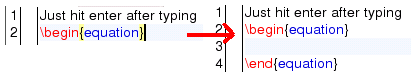
\includegraphics[width=0.5\linewidth]{snap_autocomplete}}

\caption{Automatisch aanvullen van 'Equation' omgeving}
\label{fig:autocomplete}
\end{figure}


\newpage
\subsection{$\LaTeX$ commando's} \label{sec:LaTeX commando's}

Wanneer je enkele letters typt, kan je activeren dat er een lijst verschijnt met de mogelijke commando's\index{commando}. Dit kan je doen via het menu 
\textbf{Edit \textgreater \space Complete \textgreater \space Latex Command} of via de sneltoets \textbf{Ctrl-Space}. Kile leest eerst
de letters van de huidige cursorpositie naar links en stopt bij de eerste non-letter, karakter of een backslash. Als het patroon
begint met een backslash verschijnt het aanvullingsmenu voor $\TeX$ of $\LaTeX$ commando's. Anders verschijnt het aanvullingsmenu met woordenboek functie, waar geen $\LaTeX$ commando's in staan.
Je ziet alle commando's of woorden die overeenkomen met het huidige patroon.
Je kan hier door navigeren met de navigatie-pijltjes en je kan er een selecteren met \textbf{Enter} of door te dubbelklikken.

\begin{figure}[H]
 \center{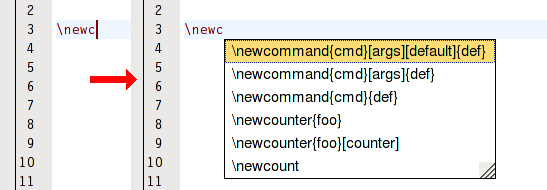
\includegraphics[width=0.5\linewidth]{complete_cmd1}}
\caption{Menu met commando's}
\label{fig:autocommands}
\end{figure}

Wanneer je op de \textbf{Backspace} knop drukt, wordt de laatst letter van je patroon verwijderd, en kan de aanvullingslijst groter worden.
Aan de andere kant, als je een andere letter typt, wordt het patroon uitgebreid, maar wordt de zichtbare lijst met woorden kleiner.
\\
Als je beslist om geen suggestie te kiezen, kan je dit venster verlaten met \textbf{Esc}.
\\
Je zal merken dat alle commando's worden geschreven met een korte beschrijving van de parameters. Deze beschrijvingen
zijn natuurlijk ingekort wanneer je een commando\index{commando} selecteerd. Optioneel kan je Kile bullets laten invoegen, zodat je gemakkelijk
kan springen naar deze positie's met \textbf{Edit \textgreater \space Bullets \textgreater \space Next Bullet}. Hier kan je de parameters\index{parameters} invoegen die je wilt.

\begin{figure}[H]
 \center{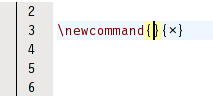
\includegraphics[width=0.5\linewidth]{complete_cmd2}}
\caption{Commando met parameters}
\label{fig:autoparam}
\end{figure}

Ga naar \textbf{Settings \textgreater \space Configure Kile... \textgreater \space Kile+Complete} om een of meerdere van deze lijsten te configureren.
Je kan kiezen uit verschillende woordenlijsten voor $\TeX$ en $\LaTeX$ commando's en een woordenboekmodus voor normale woorden.

\subsection{Afkortingen} \label{sec:Afkortingen}

Kile ondersteunt door de gebruiker ingestelde lijsten van afkortingen, welke worden vervangen op vraag van langere strings\index{strings}. Ga naar
\textbf{Settings \textgreater \space Configure Kile... \textgreater \space Kile+Complete} om een of meerdere van deze lijsten te configureren.

\newpage
\subsection{Speciale tekens} \label{sec:Speciale tekens}
Het is in $\LaTeX$ vaak goed om je accenten niet meteen in de tekst te typen.
Het zou wel eens kunnen dat accenten en andere tekens veranderen in rare tekentjes of vraagtekens. Het is beter om accenten aan te geven met $\LaTeX$ code.
Hier is een overzicht voor accenten voor de letter 'e'.

\begin{center}
 \begin{tabular}{ | l | l |}
 \hline
  \textbf{Code} & \textbf{Resultaat} \\ \hline
  $\backslash `` e $ & \"e \\ \hline
  $\backslash ' e $ & \'e \\ \hline
  $\backslash ` e $ & \`e \\ \hline 
\end{tabular}
\end{center}
\label{tab:Speciale tekens}



\newpage

\textsc{\Large Bijlage}
\section{Mail instellen met Mutt} \label{sec:Mail instellen met Mutt}

\subsection{Installatie} \label{sec:Installatie}

Het installeren van Mutt kan via \textbf{System \textgreater \space Administration \textgreater \space Synaptic Package Manager} of
via het uitvoeren van volgende commando:
\begin{lstlisting}
 sudo apt-get install mutt
\end{lstlisting}
Na het installeren krijg je de keuze tussen:

\subsection{Configuratie} \label{sec:Configuratie}

Eens Mutt ge\"installeerd is, moet je het configureren om e-mails correct te kunnen ontvangen en verzenden.
Het voordeel aan Mutt is dat bijna alles configureerbaar is. Dit kan echter ook een nadeel zijn wanneer je de instellingen verknoeit, gebruik dus met de nodige voorzichtigheid.
\\

Het configuratiebestand voor Mutt is terug te vinden in elke user z'n home-folder. Het bestand noemt \textit{.mutttrc}.
Om het te bewerken, open een terminal-venster en open het configuratiebestand met het commando:
\begin{lstlisting}
 # vim ~/.mutttrc
set imap_user = “email@gmail.com”
set imap_pass = “paswoord123”

set smtp_url = “smtp://gebruiker@smtp.gmail.com:587/”
set smtp_pass = “paswoord123”
set from = “email@gmail.com”
set realname = “Voornaam Naam”

set folder = “imaps://imap.gmail.com:993”
set spoolfile = “+INBOX”
set postponed=”+[Gmail]/Drafts”
set header_cache=~/.mutt/cache/headers
set message_cachedir=~/.mutt/cache/bodies
set certificate_file=~/.mutt/certificates

set move = no
\end{lstlisting}
De instellingen hierboven zijn de basis instellingen die nodig zijn om te starten.
In dit voorbeeld gebruiken we een Gmail account die het IMAP protocol hanteerd.
Wees zeker dat je bestand niet publiek leesbaar is, want je paswoord staat hier in.
Als je het paswoord leeg laat zal Mutt je iedere keer vragen achter je paswoord, elke keer wanneer je de applicatie opent.
Verander de instellingen hierboven naar jouw mailserver, sla het bestand op en ga aan de slag met Mutt.


\newpage
\section{Versiebeheer met GIT} \label{sec:Versiebeheer met GIT}

\subsection{Installatie} \label{sec:Installatie}

Het installeren van Git kan op verschillende manieren, de gemakkelijkste is via onderstaande commando's:
\begin{lstlisting}
 sudo apt-get install git-core
 sudo apt-get install git-doc
 sudo apt-get install git-gui
\end{lstlisting}
\subsubsection{Instellen van SSH sleutel} \label{sec:Instellen van SSH sleutel}

GIT gebruikt SSH sleutels voor een veilige verbinding te maken tussen je computer en GitHub. Deze instellen is redelijk gemakkelijk, maar verreisen enkele stappen.

\begin{enumerate}
 \item \textbf{Controleer SSH sleutels}: Controleer als er al bestaande SSH sleutels aanwezig zijn op je computer:
  \begin{lstlisting}
   cd ~/.ssh
  \end{lstlisting}
Indien ``No such file or directory'' ga naar \textbf{stap 3}.

\item \textbf{Verwijder bestaande sleutels en sla deze op} \\
Omdat er al een SSH folder bestaat, sla de oude op in een andere map en verwijder deze uit de SSH folder.

\begin{lstlisting}
 ls
 mkdir key_backup
 cp id_rsa* key_backup
 rm id_rsa*
\end{lstlisting}

\item \textbf{Genereer een nieuwe sleutel} \\
Om een nieuwe sleutel te genereren, geef onderstaande code in. Gebruik de standaardinstellingen wanneer gevraagd wordt om een bestand in te geven voor de sleutel op te slaan (druk op enter).
\begin{lstlisting}
 ssh-keygen -t rsa -C "email@adres.be"
\end{lstlisting}

Hierna moet je een passphrase ingeven. Hierna krijg je volgend resultaat:

\begin{figure}[H]
 \center{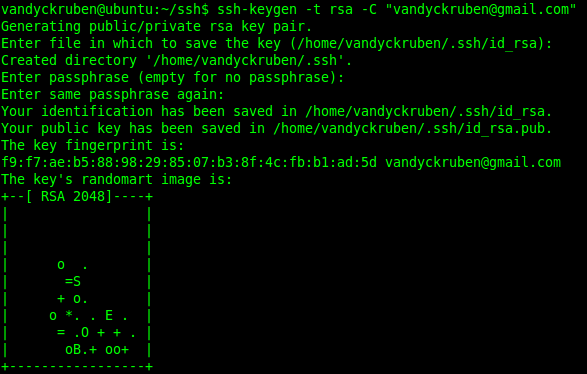
\includegraphics[width=0.5\linewidth]{GIT_ssh}}
\caption{SSH fingerprint}
\label{fig:fingerprint}
\end{figure}

\item \textbf{Toevoegen van SSH sleutel aan GitHub} \\
Ga naar de GitHub website en klik op \textbf{Account Settings \textgreater \space SSH Keys \textgreater \space Add SSH key}.\\
Open het bestand id\_rsa.pub met een tekstbewerkingsprogramma (Bv. gedit). Dit is je publieke SSH sleutel.
Kopi\"eer de volledige inhoud van het bestand in het veld ``Key''.

\begin{figure}[H]
 \center{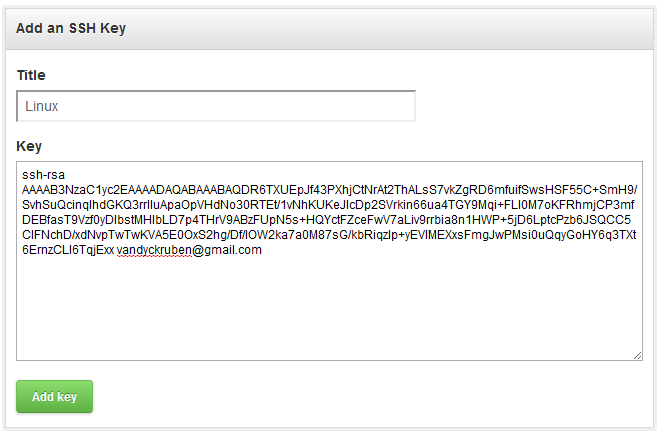
\includegraphics[width=0.5\linewidth]{ssh_key}}
\caption{De inhoud van de sleutel}
\label{fig:sshkey}
\end{figure}

\item \textbf{Testen}
Om zeker te zijn dat alles werkt kan je nu een SSH connectie leggen naar Github.
Verander ``git@github.com'' niet. Voer volgend commando uit:
\begin{lstlisting}
 ssh -T git@github.com
\end{lstlisting}
Nu zou je volgend resultaat moeten krijgen:

\begin{figure}[H]
 \center{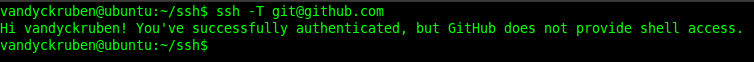
\includegraphics[width=0.7\linewidth]{ssh_auth}}
\caption{SSH verbinding}
\label{fig:sshauth}
\end{figure}



\end{enumerate}


\subsection{Persoonlijke info configureren} \label{sec:Persoonlijke info configureren}

Nu je Git hebt ge\"installeerd en de SSH sleutel hebt ingegeven op GitHub, is het tijd om je persoonlijke informatie te configureren.

\begin{enumerate}
 \item \textbf{Stel je gebruikersnaam en e-mailadres in} \\
Git houdt bij wie er iedere keer een bestand aanpast door de gebruikersnaam en het e-mailadres te controleren.
Geef de code hieronder in om deze in te stellen:
\begin{lstlisting}
 git config --global user.name "Ruben Van Dyck"
 git config --global user.email "vandyckruben@gmail.com"
\end{lstlisting}

\end{enumerate}
\subsection{Aanmaken van een repository folder} \label{sec:Aanmaken van een repository folder}

Iedere keer als je Git commit, wordt het opgeslagen in een repository. Om je project op GitHub te krijgen, moet je een GitHub repository aanmaken.

\begin{enumerate}
 \item \textbf{Maak een nieuwe repo} \\
Ga naar de website van GitHub en klik op ``New Repository''.
Vul de naam in die je wilt voor je repository map, en kies als je deze map publiek wilt delen of alleen wilt delen met mensen die jij opgeeft.
Nu kan je een README bestand gaan maken voor in je map te plaatsen.

\end{enumerate}
\newpage
\subsection{Een README aanmaken} \label{sec:Een README aanmaken}

Een README bestand is niet verplicht in een repo folder. Het is wel een goed idee om er een te hebben.
In dit bestand kan je beschrijven wat je project inhoudt, je kan er ook documentatie aan toevoegen zoals: hoe installeren, ...

\begin{enumerate}
 \item \textbf{Aanmaken van het bestand}\\
Voer volgende commando uit:

\begin{lstlisting}
 mkdir ~/Hello-World
 cd ~/Hello-World
 git init
 touch README
\end{lstlisting}

\item \textbf{Committen van het bestand}\\
Nu je een bestand hebt aangemaakt kan je er info naar keuze in plaatsen. Nu gaan we zorgen dat dit bestand beschikbaar is op github.
Voer volgende commando's uit:

\begin{lstlisting}
 git add README
 git commit -m 'Eerste commit'
 git remote add origin git@github.com:vandyckruben/Hello-World.git
 git push -u origin master
\end{lstlisting}
Als je nu kijkt op de site van GitHub zul je je README bestand zien staan.

\end{enumerate}
\newpage
\section{Bash script}
\begin{lstlisting}
 read -p 'Contactpersoon:' aanspreking;
read -p 'To (voornaam): ' vnaam;
read -p 'To (achternaam): ' anaam;
read -p 'To (e-mail adres): ' email;

#Spaties verwijderen uit namen
vnaamNospace=${vnaam// /};
anaamNospace=${anaam// /};

#het bestand de naam geven van de geadresseerde... dit doen we in 2 stappen
#eerst wisselen we van directory
cd /home/vandyckruben/Desktop/vandyckruben;
#vervolgens kopiëren we het bestand met als naam vnaam.anaam
cp Kile.pdf $vnaamNospace.$anaamNospace.pdf;

#commando om de email te verzenden via het programma mutt
#met als onderwerp "mailreviewer", naar $email en met het gekopieerde bestand als bijlage.
echo $aanspreking| mutt  -s "mailreviewer"  $email -a /home/vandyckruben/Desktop/vandyckruben/$vnaamNospace.$anaamNoscpace.pdf;
\end{lstlisting}














\newpage
\listoffigures \label{Lijst van figuren}
\newpage
\listoftables \label{Lijst van tabellen}


\newpage
\printindex \label{Index}




%----------------------------------------------------------------------------------------
%	BIBLIOGRAPHY
%----------------------------------------------------------------------------------------
Using BibTex ~\cite{BibTex}.
Setting up GitHub ~\cite{GitHub Setup}.
GitHub Making a Repository folder ~\cite{GitHub Repo}
LaTeX WikiBooks ~\cite{WikiBooks}.
A comprehensive LaTeX symbol list ~\cite{Symbol list}




\bibliography{KileBib}{}
\bibliographystyle{plain}





%----------------------------------------------------------------------------------------

\end{document}